\subsection*{Sub-microlitre delivery benchmarking}

Given the common reliance of experimental neuroscience on the delivery of small, microlitre range, liquid volumes, we sought to first benchmark how our system behaves in this regime. Since single, small volume, events are experimentally challenging to accurately measure, other systems have relied on inferring, from a large number of repetitions, the average predicted volume of a single bolus. Despite being straightforward, such a method will nevertheless be blind to trial variability, any important metric when considering psychophysical animal experiments. With this in mind, we characterized the single-trial responses of our system by developing a quantitative, computer-vision-based, assay that can provide a metric of such variability \ref{fig:PumpProtocol}. Briefly, our method relies on the videography of a small-diameter glass capillary with well-characterized, and reproducible, dimensions. By adding small amounts of food colouring to the fluid, we can reliably segment the area of the glass filled with liquid and, by assuming $Area_{pixels} \propto Volume_{mL}$, using it as a linear proxy for delivered volume. 

\begin{figure} 
	\centering
	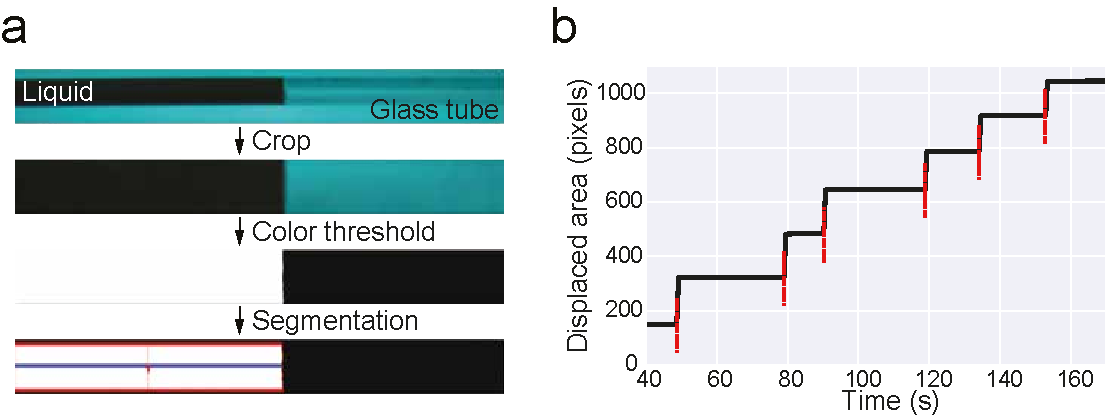
\includegraphics[width=1.0\linewidth]{Figures/Artboard 1_1.pdf}
	\caption{\textbf{Tracking small single-bolus events.}\\
		(\textbf{a}) Schematic of the computer vision algorithm followed to measure small, microlitre range, volumes. Briefly, from top to bottom, we cropped, thresholded, and segmented the area of the capillary filled with liquid. We took its area as a proxy of delivered volume. (See \hyperref[s:methods]{Methods} for further details)  \textbf{b}) Example trace of the measured area in A), as a function of time during one of the experiments. Red vertical dashed lines represent liquid delivery events.}
	\label{fig:PumpProtocol} 
\end{figure}

Using this approach, we picked four distinct liquid volumes, in a range relevant to rodent behaviour experiments 


(0.33$\mu L$ - 10$\mu L$).



 We calculated, based on the mechanical specifications of our system and mounted syringe models, the number of steps expected to achieve such volumes. Next, using the videography data, we constructed a "protocol-onset triggered"


 trace that can be used to quantify single-trial total delivered volume (during the stable phase of the trace), as well as its fluid kinetics \ref{fig:SingleStepCalibration}-a. Our procedure is thus able to provide an estimate of variability across single delivery protocols, on top of revealing a close linear relationship between theoretically predicted and delivered volume. This result held true not only across different setups (\textit{PumpA} \textit{vs.} \textit{PumpB}), but also across mounted syringes with distinct dimensions 





($10mL$ \textit{vs.} $5mL$) \ref{fig:SingleStepCalibration}-b,c. Finally, while the spread of single trial delivered volumes grew with theoretically calculated values, its coefficient of variation (standard deviation normalized by the mean) remained relatively stable in all conditions \ref{fig:SingleStepCalibration}-d,e.


\begin{figure}
	\centering
	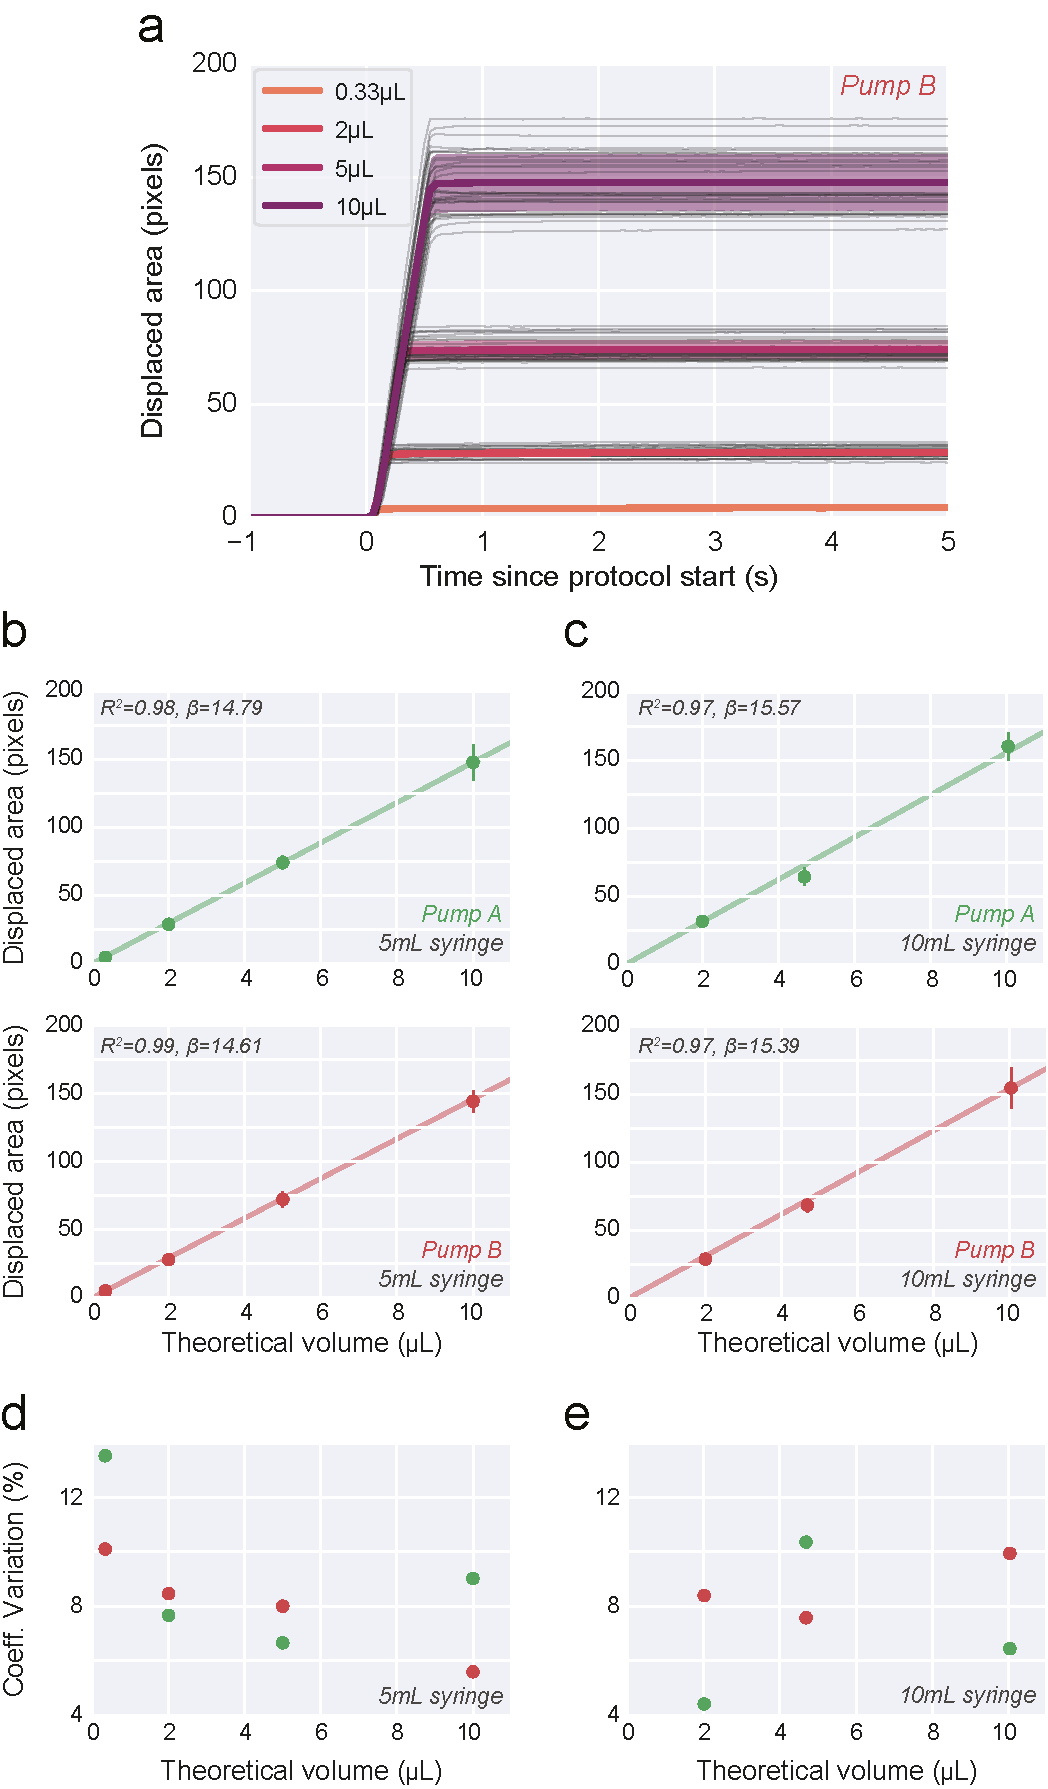
\includegraphics[width=1.0\linewidth]{Figures/Artboard 5.pdf}
	\caption{\textbf{Single-bolus protocol calibration}.\\
		(\textbf{a}) Time course of displaced area aligned on protocol onset (\textit{t} = 0) for four distinct theoretically expected delivered volumes. Thin and thick lines correspond to single trials, and averages for a given expected volume, respectively. \textbf{b, c}) Total displaced area for the four protocols. Each point shows mean$\pm$s.t.d.. across 30 replicates, per volume, in two different pumps (\textit{PumpA} and \textit{PumpB}, green and red, respectively) and using two different glass syringe models (5mL and 10mL, \textbf{b} and \textbf{c}, respectively). \textbf{d, e}) Coefficient of variation (s.t.d./mean) calculated from the data shown in \textbf{b} and \textbf{c}, respectively.}
	\label{fig:SingleStepCalibration} 
\end{figure}

\subsection*{Flow-rate modulation}
On top of providing a proxy measurement of single-trial delivered amount, our characterization method also affords the chance of measuring its single-trial time-course dynamics (\textit{i.e.} flow-rate, pixels $s^{-1}$). Theoretically, flow rate should be a function of the number of steps the driver takes per unit time. As a proof-of-concept, we performed an experiment where we varied the time between each train of pulses (protocol) and leverage our ability to measure single-trial dynamics to characterize how these changes affect the small amounts of liquid delivered per unit time \ref{fig:FlowRateControl}. Our results showed that, as predicted, the displaced area in the capillary per unit time monotonically decreases with larger intervals between protocols. While this relationship is clearly not linear, the reproducibility of such dynamics across trials affords the chance of precisely calibrating the flow-rate, for a specific system.

\begin{figure}
	\centering
	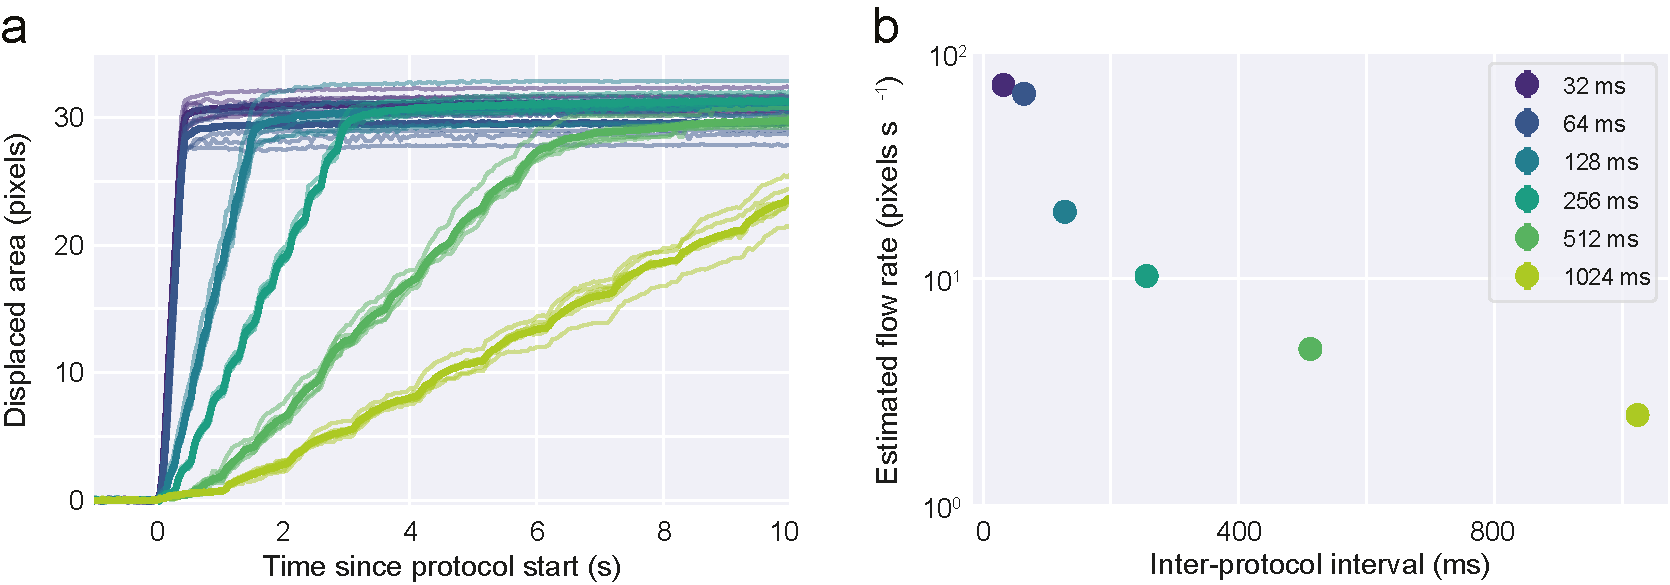
\includegraphics[width=1.0\linewidth]{Figures/Artboard 3.pdf}
	\caption{\textbf{Syringe pump affords dynamic control over the flow rate.}\\
		(\textbf{a}) Time course of delivered volume (displaced pixel area) aligned on protocol onset (\textit{t} = 0) for different inter-protocol-interval values (IPI). Thin and thick lines represent single trials, and averages, for a given IPI, respectively. (\textbf{b}). Estimated flow rate (pixels s$^{-1}$) for all tested IPI (mean$\pm$s.t.d.., n = 6 trials for each IPI).}
	\label{fig:FlowRateControl} 
\end{figure}

\subsection*{Calibration of large volumes}


After characterizing the small-bolus delivery capabilities of the system, we decided to follow a typical, and more experimentally amenable, calibration protocol. Measuring single small-volume delivery events presents a technical challenge in that equipment capable of reliably measuring such small amounts is rarely available. As a result, experimenters rely on measuring the outcome of several hundred repeats of the same protocol. While this strategy effectively blinds the researcher to inter-protocol variability, it allows the measurement of larger volumes, with smaller systematic errors, and thus the estimation of an average single-protocol delivery volume. Following such a protocol (see Methods), we demonstrate how calibration curves can be obtained from the setup, as well as validate the theoretically predicted amount of delivered volume calculated from the physical specifications of the system \ref{fig:LargeVolumeCalibration}. As predicted, both the quality  ($R^2$), and the slope ($\beta$), of the linear fit highlight the high-quality match between expected and measured volumes \ref{fig:LargeVolumeCalibration}a. Despite not being stable throughout the full range of probed delivered volumes, the coefficient of variation that results from measurements of this method is strikingly low \ref{fig:LargeVolumeCalibration}b. As a result, we strongly incentivize experiments to routinely adopt this calibration protocol.

\begin{figure}[ht] 
	\centering
	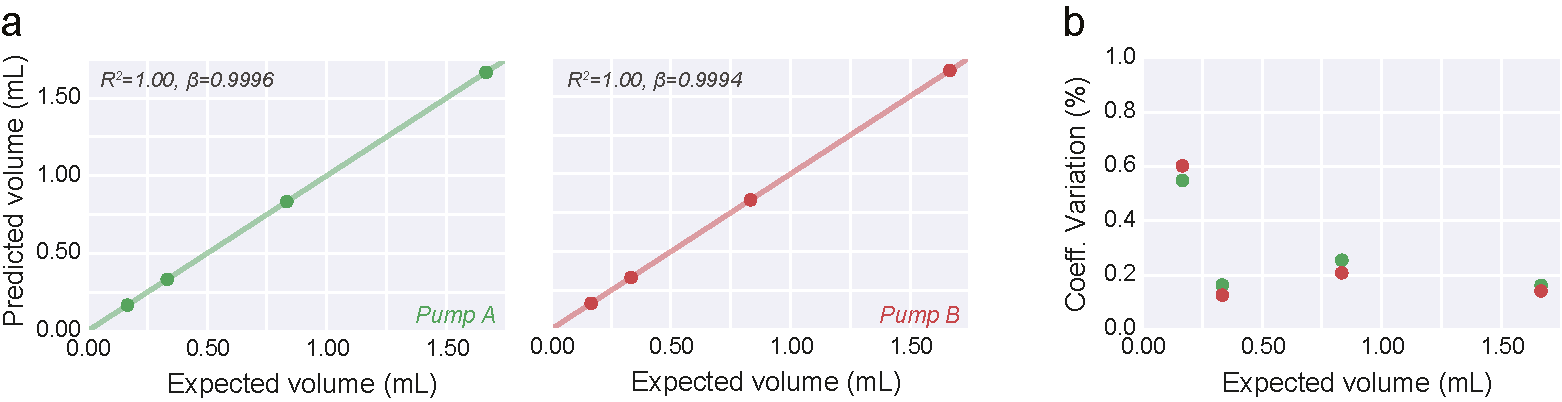
\includegraphics[width=1.0\linewidth]{Figures/Artboard 6.pdf}
	\caption{\textbf{Large volume protocol calibration}.\\
		(\textbf{a}) Delivered volume (mean$\pm$s.t.d.) across twenty performed delivery protocols for four distinct large volume amounts, in two independent pump systems (\textit{PumpA} and \textit{PumpB}, green and red, respectively). Briefly, "Predicted volume" was calculated by weighting the delivered liquid and assuming a water density of 1g/mL. "Expected Volume" was calculated using the theoretically displaced syringe volume.  $R^{2}$ and slope ($\beta$) resulting from the linear fit to the data are shown in the top-left corner. \textbf{b}) Coefficient of variation (s.t.d./mean) calculated from the data shown in \textbf{a}.}
	\label{fig:LargeVolumeCalibration} 
\end{figure}

\subsection*{Calibration stability and comparison against gravity-based systems}

We the previous section we show how calibration of the system can be achieved in an experimentally amenable fashion. Whilst such a procedure should take no more than a few minutes, it can quickly become unfeasible if several water delivery systems are routinely used simultaneously. As a result, we next benchmarked how stable the calibration values are by performing longitudinal, weekly, calibration procedures. Our data shows that, at least, up to one month after the initial procedure (\textit{Day 0}), calibration curves are identical \ref{fig:PumpVsValve}a, left.

Next, we considered the most common alternative to a syringe-pump system, in experimental behaviour neuroscience: gravity-based systems. These systems rely on having a liquid reservoir at a higher potential than the system's outlet. Such difference in potential leads to hydrostatic pressure that can be leveraged by opening and closing gates (\textit{e.g.} using valves) to control the flow of liquid through the outlet. While simpler and generally more affordable, these systems are usually subject to changes in the fluid path resistance that lead to systematic differences in delivered volume over days, and weeks. This problem can be partially circumvented by investing time on regular setup calibration and maintenance, which tends to hinder the scalability of this solution.

To compare the stability of the presented syringe pump system versus a common gravity-based system, routinely used for behaviour experiments, we decided to perform, and track, regular calibrations results of both the systems, under identical daily use, and observed how these values changed over the course of the experiment \ref{fig:PumpVsValve}.

For both systems, we followed a calibration procedure identical to the one described in the last section using volumes in a similar range. As expected, both systems show daily calibration curves consistent with a linear behaviour \ref{fig:PumpVsValve}a. However, a clear change in slope, over days, can be observed in both valves (\ref{fig:PumpVsValve}a). Using the daily calibration values, one can ask: "what much liquid volume would be delivered, had the experimenter not performed the calibration procedure, and kept using the values from Day 0" \ref{fig:PumpVsValve}b. This analysis revealed that, as opposed to the syringe pumps, gravity-based valve systems steadily drift over days. It should be noted that the general decrease in delivered volume is likely due to a drop in flow rate due to the accumulation of biofilm in the tube and valves. 

\begin{figure} 
	\centering
	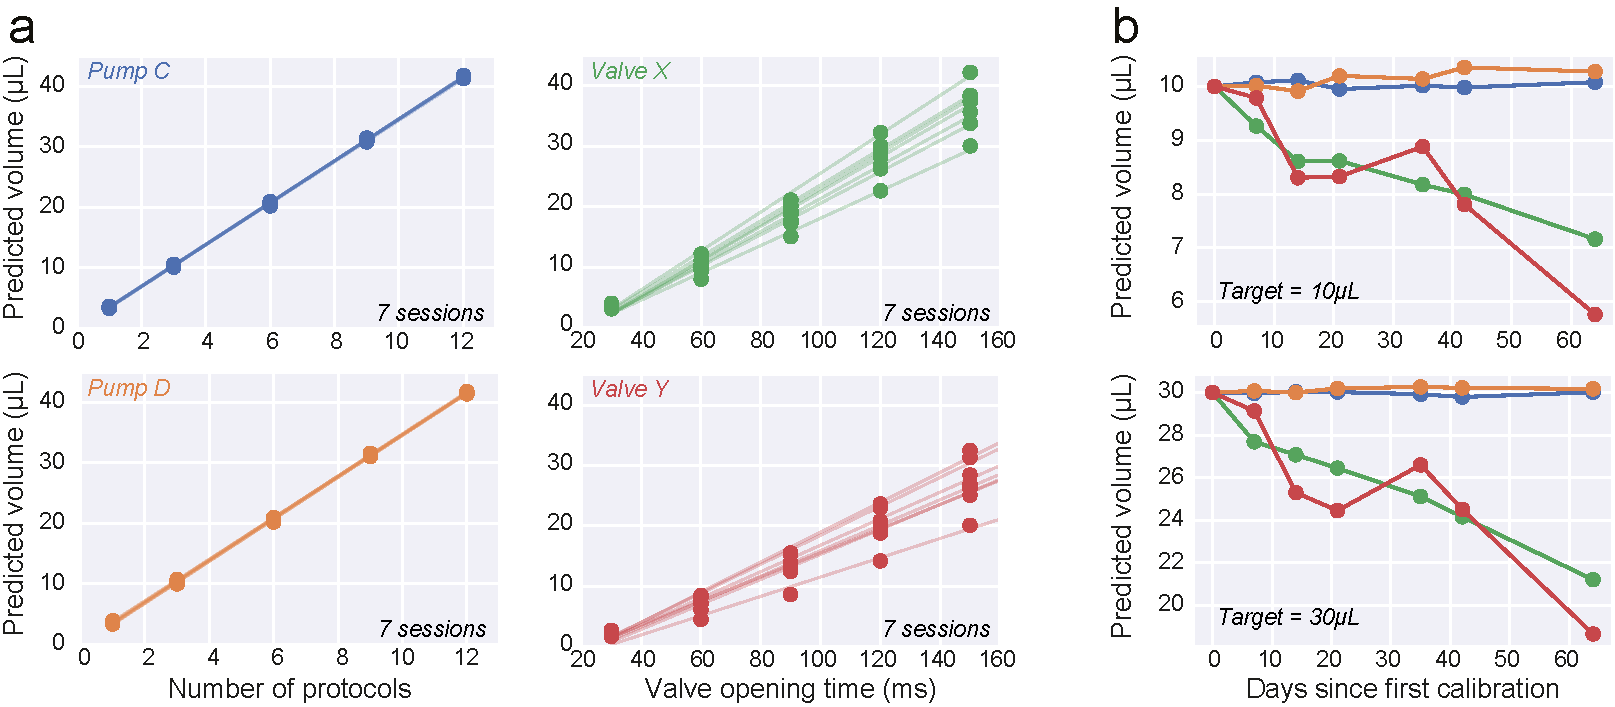
\includegraphics[width=1.0\linewidth]{Figures/Artboard 2.pdf}
	\caption{\textbf{Comparison of calibration stability between the gravity-based solution and the presented pump system.}\\
		(\textbf{a}) For each system, we followed a calibration protocol (See \hyperref[s:methods]{Methods}) wherein we measured the amount of delivered liquid as a function of the number of pre-programmed delivery protocols, or valve opening time, for the \textit{Pump} (left) and \textit{Valve} (right) solutions, respectively. Individual fits correspond to a single-day calibration protocol. For each system, we tested two devices independently (distinct colours). (\textbf{b}) Predicted delivery volume for two arbitrary volumes (10$\mu$L and 30$\mu$L, top and bottom, respectively) based on the calibration linear fits derived from A). For each day, we used the calculated fit to estimate how much volume would have been delivered had we kept the values from Day 0}
	\label{fig:PumpVsValve} 
\end{figure}


\subsection*{Experimental use cases}

Following the systematic characterization of the hereto introduced system, we next show two examples of its use in a neuroscience laboratory setting. We decided on two example experiments that highlight both the day-to-day easy of operation, but also the compatibility of the system with other existing technical methods.

In our first example, we tested rats in a two-arm bandit task, wherein delivered reward amount was parametrically varied using our system. On each block (see Methods), the amount of reward at each arm was randomly drawn from a set of five possible values. Both tested animals (N=2) appeared to be sensitive to the relative amount of reward delivered and showed a systematic preference towards the highest-reward amount option, in a way consistent with its relative difference in magnitude \ref{fig:Behavior}. Moreover, this preference quickly reversed at block transition, modulated by the relative difference between the two options, suggesting that animals did not need to rely on several trials to determine the highest-value arm.

\begin{figure}[ht] 
	\centering
	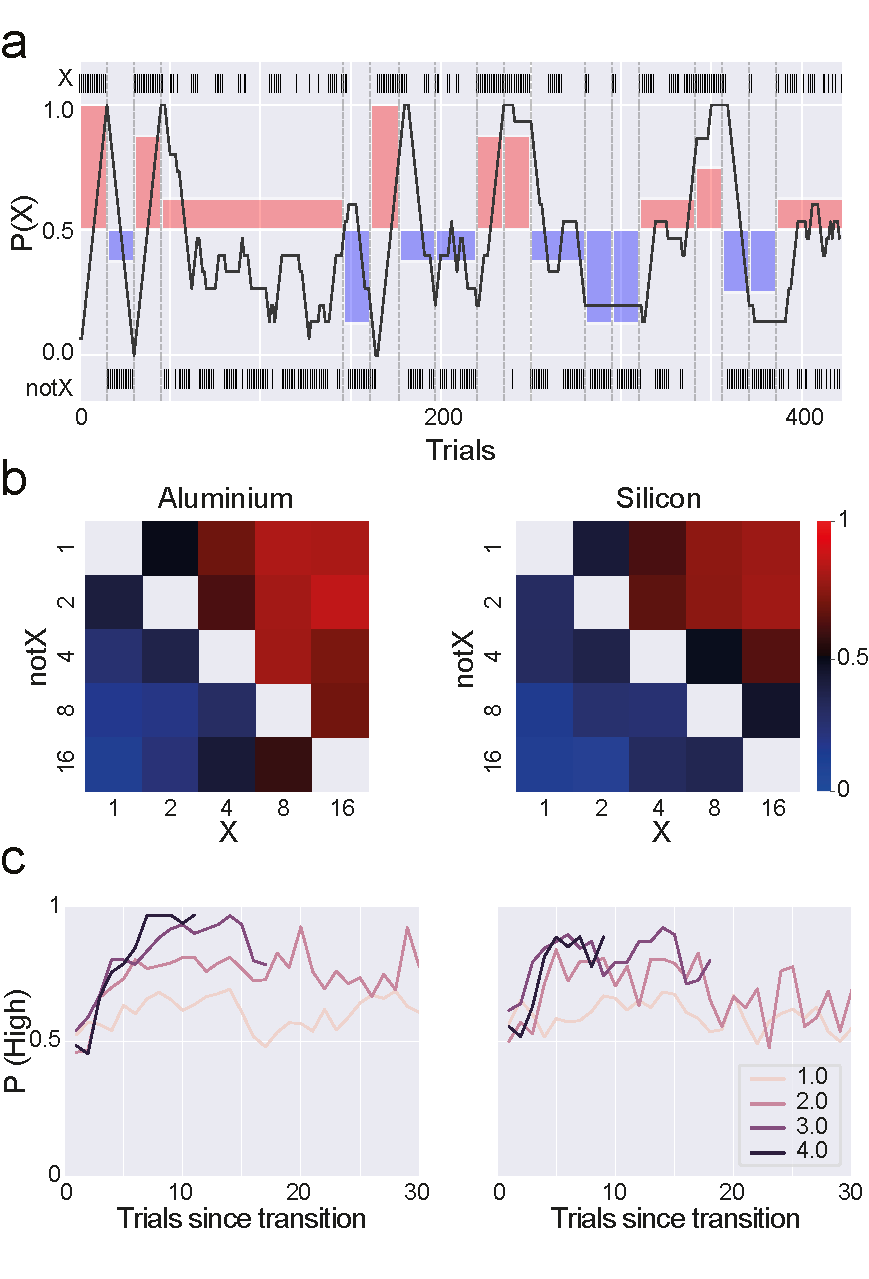
\includegraphics[width=1.0\linewidth]{Figures/Artboard 9.pdf}
	\caption{\textbf{Rats quickly reserve choice preference on delivered liquid reward amount }.\\
		(\textbf{a}) Example session. Animals alternate between the two available choices ("X" and "notX", top and bottom rasters, respectively) in a way that appears consistent with the highest-value choice (shaded area). Thick dark line depicts the probability of choosing "X" in a rolling window of 15 trials. (\textbf{b}) Probability of choosing reward giving nose-port X as a function of the possible reward amount combinations given by each nose-port. Values in the heatmap axes are the number of protocols given on each reward delivery, by each reward nose-port (X and notX). (\textbf{c}) Probability of choosing the highest rewarded side over the trials following block transition. Lines correspond to the absolute value of the difference between rewards at each nose-port in logarithmic units (base 2). The highest the difference between the two rewards available on a particular block, the sooner animals converge to the highest rewarded nose-port, [suggesting the need for fewer reward samples (trials) as the difference between rewards increases]. }
	\label{fig:Behavior} 
\end{figure}

Finally, given the current reliance of the Neuroscience field on electrophysiological recordings, it is pertinent to ascertain the compatibility of the described system with such techniques. Previous reports of induced artefacts stemming from stepper-motor operation near these systems \citep{Amarante2019}. As a result, we performed acute electrophysiological recordings from a mouse's brain (Methods) while simultaneously operating the syringe pump \ref{fig:Ephys}. 
We leveraged one of the digital outputs in the board to send a pulse on each "STEP" instruction, thus providing precise sub-millisecond alignment to the activity traces. 
Our data showed a clear absence of artefacts aligned to, or surrounding, each pulse, while still preserving easily identifiable single-unit spiking activity, thereby validating the use of the presented syringe pump system during electrophysiological recordings.

\begin{figure}[ht] 
	\centering
	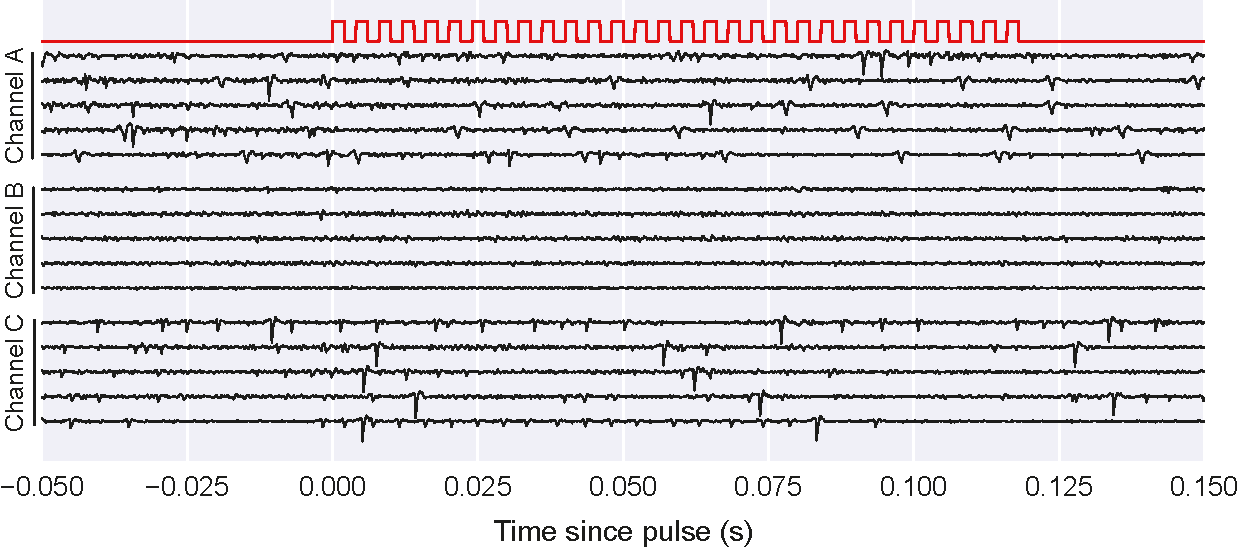
\includegraphics[width=1.0\linewidth]{Figures/Artboard 7.pdf}
	\caption{\textbf{Compatibility with electrophysiological recordings}.\\
	Example single trial traces (four trials) for three simultaneously recorded channels (A-C) aligned to the start of a protocol of several pulses (red trace). See Methods for further details. Notice the presence of spiking activity in Channels A and B, along with the lack of any clearly identified stepper-motor-induced electrical artefact.}	
	\label{fig:Ephys}
\end{figure}




